% !TEX root = C:/Users/piyus/knowledge/Project_Specific_Knowledge/public/fm_radio/stages/input_stage/input_stage.tex
\documentclass[12pt, letterpaper]{article}

\usepackage{graphicx}
\graphicspath{ {C:/Users/piyus/knowledge/Project_Specific_Knowledge/public/fm_radio/stages/input_stage/pictures} }

\title{Input Stage Notes}
\author{Piyush Sud}
\date{9/25/2024}
\begin{document}
\maketitle

\pagebreak

\section{High Level Design}
\begin{itemize}
    \item Filters before the mixer have a relatively large BW. Most filtering is done at the IF, so the Q value requirement is lower.
    \item https://electronics.stackexchange.com/questions/153830/should-i-use-a-passive-or-an-active-filter
    \item Plan to use a simple LC circuit with a variable capacitor for tuning.
    \item But how do we tune the mixer and input filter together using a single knob?
    \item It seems like we can use a dual gang capacitors or control the voltage of multiple varactors using a microcontroller.
    \item However, according to perplexity, most car radios just have a fixed input filter which allows frequencies of 88 MHz to 108 MHz to pass, while the specific band frequency is controlled by the mixer.
    \item Therefore, we can just use a LC bandpass filter with a low cutoff of 88 MHz and high cutoff of 108 MHz. Since most of the filtering is done at the IF we don't really need to worry about the Q value of this filter.
\end{itemize}

\section{Detailed Filter Design}
\begin{itemize}
    \item I found this online tool to design filters for me. I could have designed it myself since this is a simple filter, but it exports the SPICE model and everything so it makes it easier.
    \item https://markimicrowave.com/technical-resources/tools/lc-filter-design-tool/
    \item In FM modulation, the transmitted signal is a function of the baseband signal and the carrier,
    \[
        x(t) = cos(w_ct + \phi(t))
    \]
    \item The frequency of this signal is given by the deriviative of the phase, or 
    \[
        f = w_c + \frac{d\phi(t)}{dt}
    \]
    \item The fourier transform of \(\frac{d\phi(t)}{dt}\) is \(2 \pi j\omega\frac{d\phi(\omega)}{d\omega}\), which is proportional to group delay. Therefore, I need to choose a filter with a near constant group delay. 
    \item A bessel filter tends to have the smallest group delay out of most popular passive filter types, so let's choose that.
\end{itemize}

\section{Results}
Here is the simulation of a second order bandpass filter:
\begin{figure}[h]
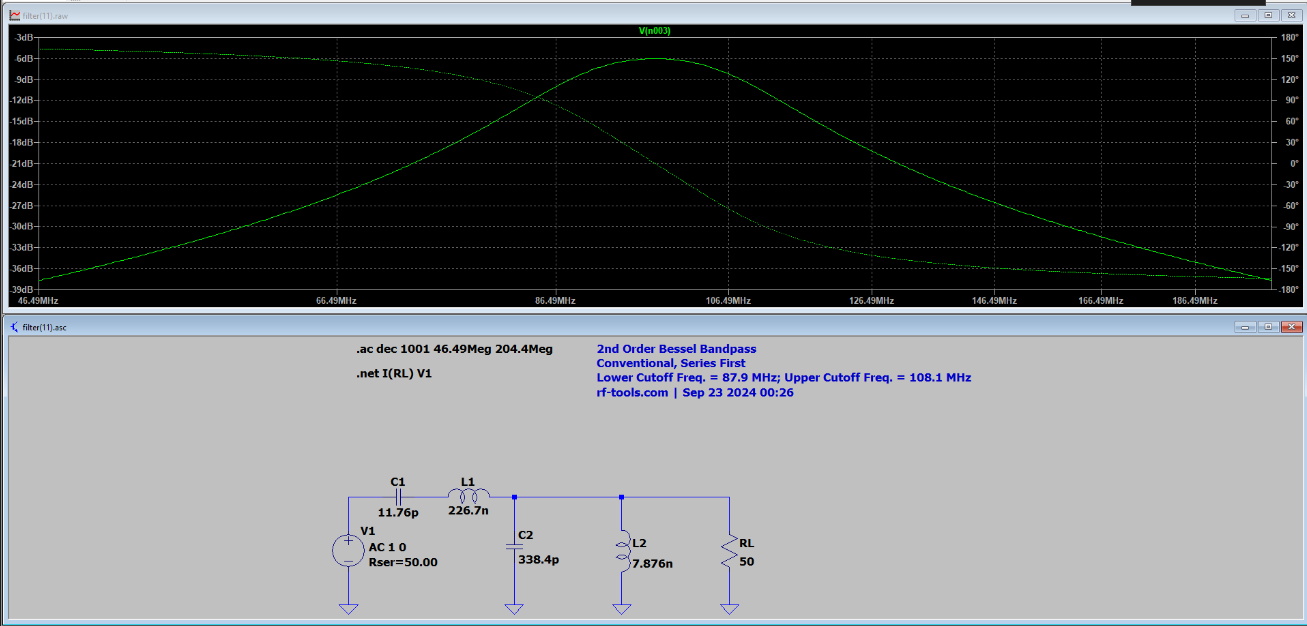
\includegraphics[width=\textwidth]{filter_sim_ideal}
\end{figure}

\clearpage

Here is the same simulation with real component values from digikey:
\begin{figure}[h]
    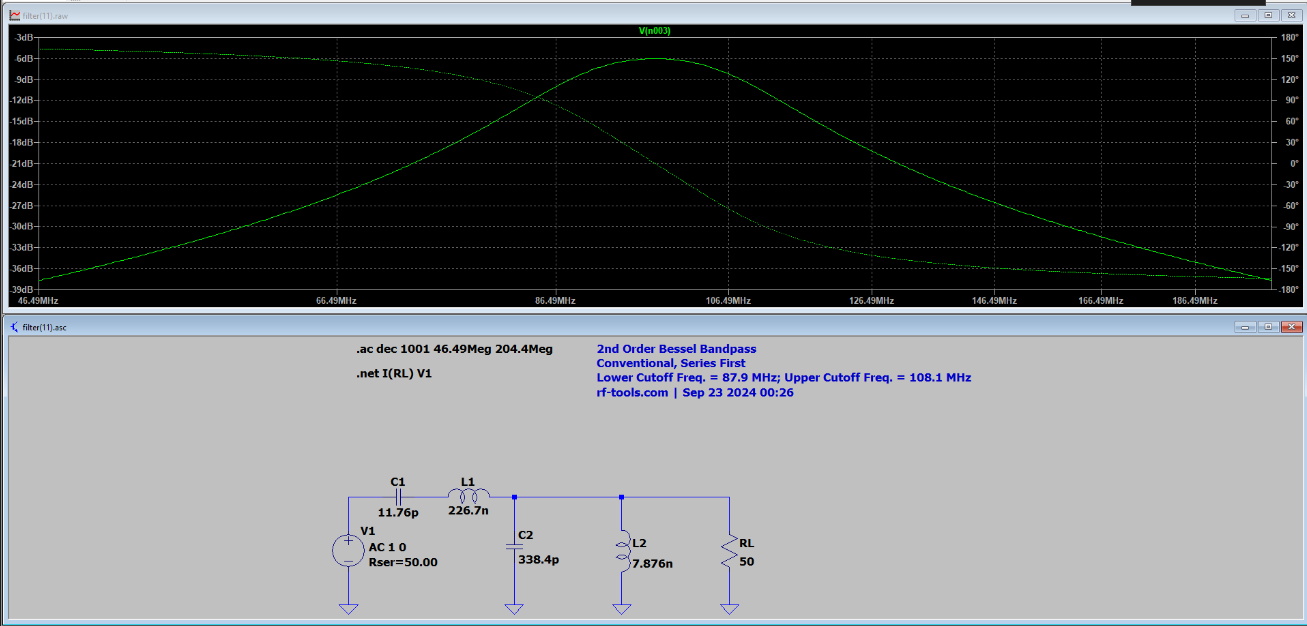
\includegraphics[width=\textwidth]{filter_sim_ideal}
\end{figure}

\end{document}